\section{Представления}

\subsection{Создание представления}
\textbf{Формулировка задания на русском языке.}

Создать представление, в котором необходимо для каждой коровы
подсчитать количество лактаций и количество рационов,
по которым она питалась.

Команда создания представления на языке SQL приведена в листинге \ref{lst:create_view}.

\begin{lstlisting}[caption={Создание представления}, label={lst:create_view}]
CREATE VIEW Cow_Lactation_Diet_Count AS
SELECT Cow.id_Cow, COUNT(DISTINCT Lactation.id_Lactation) AS lactation_count,
COUNT(DISTINCT Diet.id_Diet) AS diet_count
FROM Cow
LEFT JOIN Lactation ON Lactation.id_Cow = Cow.id_Cow
LEFT JOIN Nutrition ON Nutrition.id_Cow = Cow.id_Cow
LEFT JOIN Feeding_plan ON Feeding_plan.id_Feeding_plan = Nutrition.id_Feeding_plan
LEFT JOIN Diet ON Diet.id_Diet = Feeding_plan.id_Diet
GROUP BY Cow.id_Cow;
\end{lstlisting}

На рисунке \ref{fig:create_view_res} продемонстрирована часть таблицы ---
результат выполнения команды создания представления.
\begin{figure}[H]
    \centering
    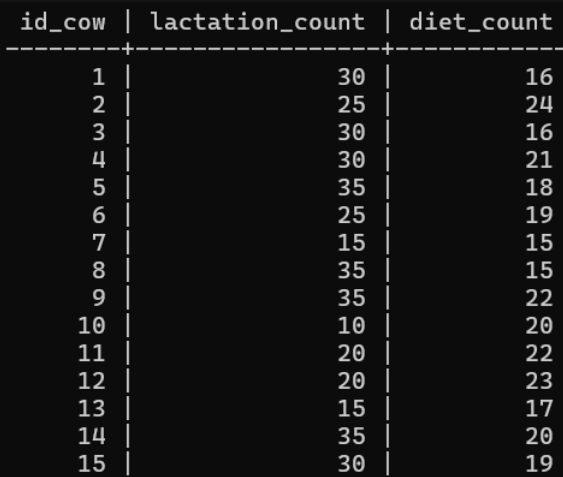
\includegraphics[width=0.5\linewidth]{images/create_view_res.png}
    \caption{Результат выполнения команды создания представления}
    \label{fig:create_view_res}
\end{figure}

На рисунке \ref{fig:create_view_exp}
продемонстрирован план выполнения SQL-запроса, лежащего в основе созданного представления.
\begin{figure}[H]
    \centering
    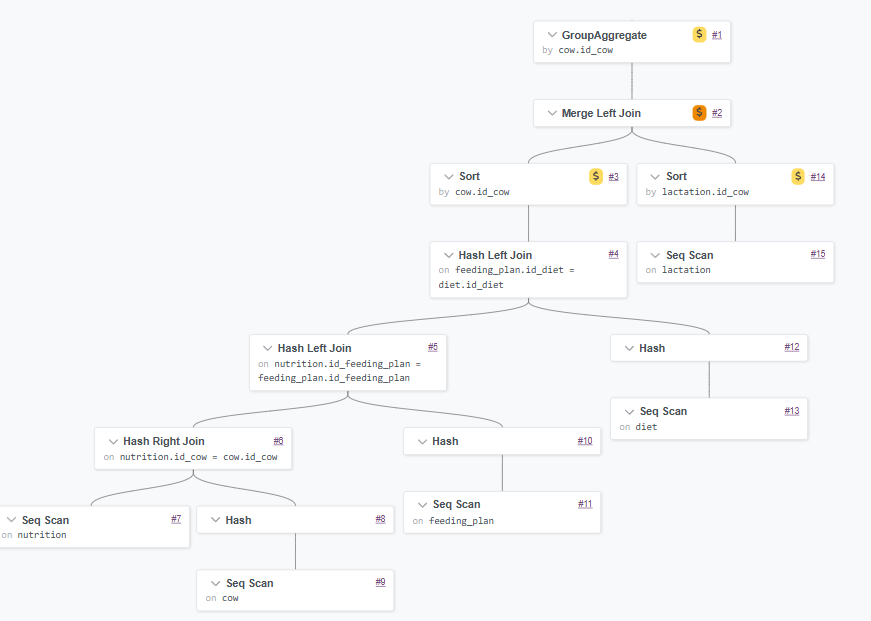
\includegraphics[width=\linewidth]{images/create_view_exp.png}
    \caption{Графическое представление последовательности выполнения запроса при создании представления}
    \label{fig:create_view_exp}
\end{figure}


\textbf{Текстовое объяснение последовательности выполнения запроса, лежащего
в основе создания  представления.}

В запросе сначала осуществляется обращение к базовой таблице \\\texttt{Cow}.
Затем к ней последовательно присоединяются таблицы \texttt{Lactation, Nutrition, Feeding\_plan} и
\texttt{Diet} с использованием оператора левого внешнего соединения (\texttt{LEFT JOIN}).
После объединения данных строки группируются по уникальному идентификатору коровы (\texttt{Cow.id\_Cow})
с помощью \texttt{GROUP BY}. Для каждой группы (каждой коровы) с помощью агрегатной функции
\texttt{COUNT} и ключевого слова \texttt{DISTINCT} вычисляется количество уникальных записей
лактаций и уникальных рационов. Итоговый результат сохраняется в базе данных как виртуальная
таблица (представление) под именем \texttt{Cow\_Lactation\_Diet\_Count}.

\textbf{Реляционная формула команды.}
\[
    \text{Cow\_Lactation\_Diet\_Count} \leftarrow \mathcal{G}_{\substack{
        \text{Cow.id\_Cow}, \\
        \text{COUNT(DISTINCT Lactation.id\_Lactation)} \rightarrow \text{lactation\_count}, \\
        \text{COUNT(DISTINCT Diet.id\_Diet)} \rightarrow \text{diet\_count}
    }} (
\]
\[
    \text{Cow} \overset{\text{LEFT}}{\bowtie}_{\text{Cow.id\_Cow}=\text{Lactation.id\_Cow}} \text{Lactation}
\]
\[
    \overset{\text{LEFT}}{\bowtie}_{\text{Cow.id\_Cow}=\text{Nutrition.id\_Cow}} \text{Nutrition}
\]
\[
    \overset{\text{LEFT}}{\bowtie}_{\text{Nutrition.id\_Feeding\_plan}=\text{Feeding\_plan.id\_Feeding\_plan}} \text{Feeding\_plan}
\]
\[
    \overset{\text{LEFT}}{\bowtie}_{\text{Feeding\_plan.id\_Diet}=\text{Diet.id\_Diet}} \text{Diet}
    )
\]

\subsection{Запрос 1}
\textbf{Формулировка запроса 1 на русском языке.}

Подсчитать количество коров, у которых было больше 2 лактаций.

Код запроса на языке SQL представлен в листинге \ref{lst:запрос_1}.

\begin{lstlisting}[caption={Запрос 1}, label={lst:запрос_1}]
    SELECT COUNT(*) FROM Cow_Lactation_Diet_Count WHERE lactation_count > 2;
\end{lstlisting}

На рисунке \ref{1view_res} продемонстрирован результат выполнения запроса.

\begin{figure}[H]
    \centering
    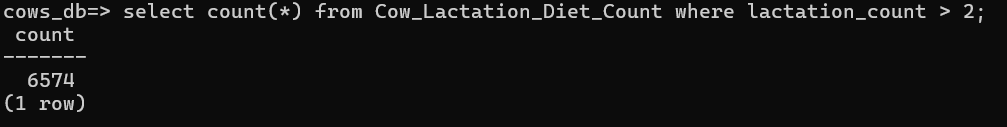
\includegraphics[width=\linewidth]{images/1view_res.png}
    \caption{Результат выполнения запроса 1}
    \label{1view_res}
\end{figure}

На рисунке \ref{1view_exp}
продемонстрировано графическое представление последовательности выполнения запроса 1.
\begin{figure}[H]
    \centering
    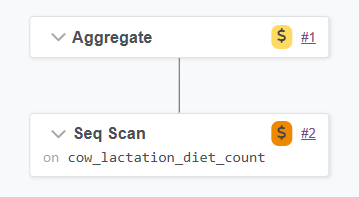
\includegraphics[width=0.6\linewidth]{images/1view_exp.png}
    \caption{Графическое представление последовательности выполнения запроса 1}
    \label{1view_exp}
\end{figure}

\textbf{Текстовое объяснение последовательности выполнения запроса 1.}

В запросе осуществляется обращение к ранее созданному представлению\\
\texttt{Cow\_Lactation\_Diet\_Count}.
Сначала с помощью оператора \texttt{WHERE} отфильтровываются записи,
оставляя только те строки, в которых значение атрибута \texttt{lactation\_count}
(количество лактаций) строго больше двух.
Затем для полученного набора данных применяется агрегатная функция \texttt{COUNT},
которая подсчитывает итоговое количество строк (коров),
удовлетворяющих заданному условию.

\textbf{Реляционная формула запроса.}
\[
    \mathcal{G}_{\text{COUNT(*)} \rightarrow \text{cow\_count}} (
\]
\[
    \sigma_{\text{lactation\_count} > 2} (
    \]
    \[
    \text{Cow\_Lactation\_Diet\_Count}))
\]

\subsection{Запрос 2}

\textbf{Формулировка запроса 2 на русском языке.}

Для каждой коровы вывести возраст, количество лактаций, количество рационов
и кормов по которым она питалась.

Код запроса на языке SQL представлен в листинге \ref{lst:запрос_2}.

\begin{lstlisting}[caption={Запрос 2}, label={lst:запрос_2}]
    SELECT Cow.id_Cow, Cow.Age, Cow_Lactation_Diet_Count.lactation_count,
    Cow_Lactation_Diet_Count.diet_count, COUNT(DISTINCT Feeds.id_Feeds) AS feed_count
    FROM Cow_Lactation_Diet_Count
    JOIN Cow ON Cow.id_Cow = Cow_Lactation_Diet_Count.id_Cow
    LEFT JOIN Nutrition ON Nutrition.id_Cow = Cow.id_Cow
    LEFT JOIN Feeding_plan ON Feeding_plan.id_Feeding_plan = Nutrition.id_Feeding_plan
    LEFT JOIN Feeds ON Feeds.id_feeds = Feeding_plan.id_feeds
    GROUP BY Cow.id_Cow, Cow.Age, Cow_Lactation_Diet_Count.lactation_count, Cow_Lactation_Diet_Count.diet_count;
\end{lstlisting}

На рисунке \ref{2view_res} продемонстрирован результат выполнения запроса \\(часть таблицы).

\begin{figure}[H]
    \centering
    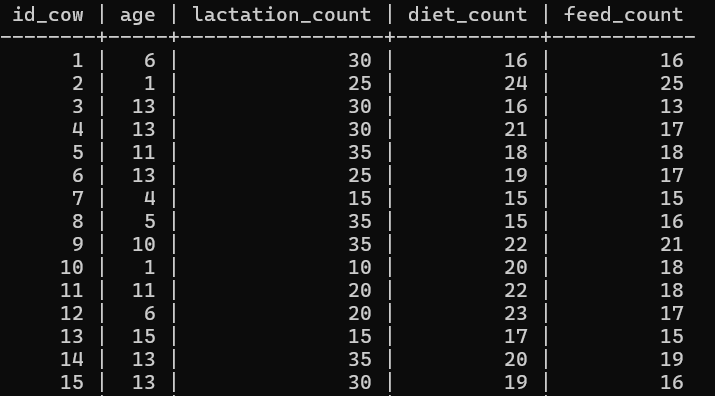
\includegraphics[width=\linewidth]{images/2view_res.png}
    \caption{Результат выполнения запроса 2}
    \label{2view_res}
\end{figure}

На рисунке \ref{2view_exp}
продемонстрировано графическое представление последовательности выполнения запроса 2.
\begin{figure}[H]
    \centering
    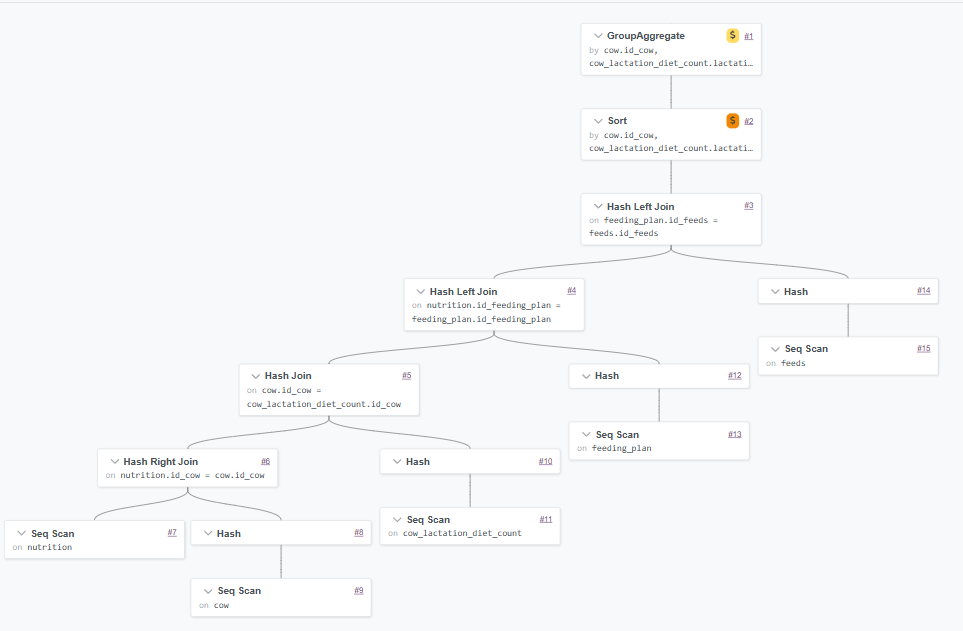
\includegraphics[width=\linewidth]{images/2view__exp.png}
    \caption{Графическое представление последовательности выполнения запроса 2}
    \label{2view_exp}
\end{figure}

\textbf{Текстовое объяснение последовательности выполнения запроса 2.}

В запросе осуществляется обращение к представлению \\\texttt{Cow\_Lactation\_Diet\_Count},
к которому с помощью внутреннего соединения (\texttt{JOIN})
присоединяется базовая таблица \texttt{Cow}.
Затем к полученному результату последовательно присоединяются таблицы
\texttt{Nutrition, Feeding\_plan} и \texttt{Feeds} с использованием оператора
левого внешнего соединения (\texttt{LEFT JOIN}).
После объединения данных строки группируются по идентификатору и возрасту коровы,
а также по количествам лактаций и рационов, полученным из представления.
В завершение для каждой группы с помощью агрегатной функции \texttt{COUNT} и
ключевого слова \texttt{DISTINCT} вычисляется количество уникальных идентификаторов
кормов (\texttt{feed\_count}).

\textbf{Реляционная формула запроса.}
\[
    \mathcal{G}_{\substack{
        \text{Cow.id\_Cow, Cow.Age}, \\
        \text{Cow\_Lactation\_Diet\_Count.lactation\_count}, \\
        \text{Cow\_Lactation\_Diet\_Count.diet\_count}, \\
        \text{COUNT(DISTINCT Feeds.id\_Feeds)} \rightarrow \text{feed\_count}
    }} (
\]

\[
    \text{Cow\_Lactation\_Diet\_Count} \bowtie_{\text{Cow\_Lactation\_Diet\_Count.id\_cow}=\text{Cow.id\_cow}} \text{Cow}
\]
\[
    \overset{\text{LEFT}}{\bowtie}_{\text{Cow.id\_cow}=\text{Nutrition.id\_cow}} \text{Nutrition}
\]
\[
    \overset{\text{LEFT}}{\bowtie}_{\text{Nutrition.id\_Feeding\_plan}=\text{Feeding\_plan.id\_Feeding\_plan}} \text{Feeding\_plan}
\]
\[
    \overset{\text{LEFT}}{\bowtie}_{\text{Feeding\_plan.id\_feeds}=\text{Feeds.id\_feeds}} \text{Feeds})
\]

